\chapter{\label{cap:plan}Plan de trabajo}

Lo siguiente en el desarrollo de mi protocolo es el montaje del cambiador de fase alrededor de la cámara de ciencia, la implementación de la trampa dipolar, optimizar las mediciones y realizar el análisis para caracterizar los pulsos de luz que pasan por un medio en EIT, finalmente comparar con simulaciones.

\section{\label{sec:montajeCambiadorFase}Montaje del cambiador de fase}

Utilizando el cambiador de fase podremos mandar, a la vez, dos pulsos de luz que atraviesen el medio atómico. La figura~\ref{fig:montajeCambiadorFase} muestra el plan de montaje de la optomecánica de nuestro dispositivo cambiador de fase con moduladores acusto-ópticos. Primero enviamos un haz a nuestro dispositivo, cuya frecuencia es la misma que la frecuencia del estado base al primer estado excitado del Rb, se crean los dos brazos de luz del interferómetro, uno de ellos con la frecuencia cambiada; luego ambos haces se acoplan a la misma fibra óptica que los manda hacia la nube de átomos en condiciones de EIT, el haz con la frecuencia inicial experimenta la dispersión del medio pues su frecuencia está dentro de la ventana de transparencia (fig.~\ref{fig:eitDispersion}), mientras que al otro haz le cambiamos la frecuencia lo suficiente para que esté suficientemente alejado de dicha ventana y que no sea absorbido por el medio. Una vez pasan el medio, ambos haces se acoplan a otra fibra que los dirige a la segunda parte del dispositivo cambiador para regresar a la frecuencia inicial. Entonces realizamos mediciones de detección homodina.

\begin{figure}[H]
\centering
\begin{minipage}{0.91\textwidth}
\centering
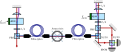
\includegraphics[width=0.95\textwidth]{montajeCambiadorFase}
\caption{\label{fig:montajeCambiadorFase}Plan para implementar nuestro dispositivo cambiador de fase. En este montaje ambos brazos del interferómetro siguen el mismo camino y la nube atómica introduce un cambio de fase en el haz cuya frecuencia está en la ventana de transparencia EIT.}
\end{minipage}
\end{figure}

\section{\label{sec:trampaDipolar}Trampa dipolar}

En la dirección de incrementar la densidad óptica de la nube primero tenemos que poner en marcha el bombeo óptico. Como ya mencioné, solamente nos faltan unos circuitos para variar el campo generado por las bobinas de forma rápida. Lo siguiente es la implementación de una trampa dipolar que, a su vez, nos permitirá cambiar la forma de la nube. Una vez construyamos la trampa dipolar, hagamos las optimizaciones y caracterizaciones pertinentes, realizaremos nuevamente experimentos del cambio de fase de la luz ahora con mayor $\OD$.

\section{\label{sec:luzLenta}Luz lenta}

Utilizando el mismo montaje del cambiador de fase, podremos mandar un haz muy lejos de resonancia para que no sea absorbido ni dispersado por el medio, y otro que sí experimente una disminución en su velocidad de grupo. Con ayuda de un generador de funciones se enviarán pulsos con perfil temporal gaussiano para probar si, de esta forma, logramos medir el retraso de la luz o si tenemos que probar con otro tipo de pulsos. Las mediciones del retraso se harán para varias intensidades del haz de control para caracterizar la nube de átomos. Asimismo, con la trampa dipolar podremos modificar la densidad atómica y el largo $L$ que la luz atraviesa dentro de la nube y realizar mediciones con estos cambios en los parámetros.